\documentclass[man,a4paper,noextraspace,apacite]{apa6}\usepackage[]{graphicx}\usepackage[]{color}
%% maxwidth is the original width if it is less than linewidth
%% otherwise use linewidth (to make sure the graphics do not exceed the margin)
\makeatletter
\def\maxwidth{ %
  \ifdim\Gin@nat@width>\linewidth
    \linewidth
  \else
    \Gin@nat@width
  \fi
}
\makeatother

\definecolor{fgcolor}{rgb}{0.345, 0.345, 0.345}
\newcommand{\hlnum}[1]{\textcolor[rgb]{0.686,0.059,0.569}{#1}}%
\newcommand{\hlstr}[1]{\textcolor[rgb]{0.192,0.494,0.8}{#1}}%
\newcommand{\hlcom}[1]{\textcolor[rgb]{0.678,0.584,0.686}{\textit{#1}}}%
\newcommand{\hlopt}[1]{\textcolor[rgb]{0,0,0}{#1}}%
\newcommand{\hlstd}[1]{\textcolor[rgb]{0.345,0.345,0.345}{#1}}%
\newcommand{\hlkwa}[1]{\textcolor[rgb]{0.161,0.373,0.58}{\textbf{#1}}}%
\newcommand{\hlkwb}[1]{\textcolor[rgb]{0.69,0.353,0.396}{#1}}%
\newcommand{\hlkwc}[1]{\textcolor[rgb]{0.333,0.667,0.333}{#1}}%
\newcommand{\hlkwd}[1]{\textcolor[rgb]{0.737,0.353,0.396}{\textbf{#1}}}%

\usepackage{framed}
\makeatletter
\newenvironment{kframe}{%
 \def\at@end@of@kframe{}%
 \ifinner\ifhmode%
  \def\at@end@of@kframe{\end{minipage}}%
  \begin{minipage}{\columnwidth}%
 \fi\fi%
 \def\FrameCommand##1{\hskip\@totalleftmargin \hskip-\fboxsep
 \colorbox{shadecolor}{##1}\hskip-\fboxsep
     % There is no \\@totalrightmargin, so:
     \hskip-\linewidth \hskip-\@totalleftmargin \hskip\columnwidth}%
 \MakeFramed {\advance\hsize-\width
   \@totalleftmargin\z@ \linewidth\hsize
   \@setminipage}}%
 {\par\unskip\endMakeFramed%
 \at@end@of@kframe}
\makeatother

\definecolor{shadecolor}{rgb}{.97, .97, .97}
\definecolor{messagecolor}{rgb}{0, 0, 0}
\definecolor{warningcolor}{rgb}{1, 0, 1}
\definecolor{errorcolor}{rgb}{1, 0, 0}
\newenvironment{knitrout}{}{} % an empty environment to be redefined in TeX

\usepackage{alltt}
\usepackage{apacite}

\title{Always Use the Separate Variances t Test for Two Independent Groups}
\shorttitle{Separate Variances t Test}
\author{Joshua D. Wondra and Richard Gonzalez}
\affiliation{University of Michigan}

\abstract{This is an abstract}
\keywords{t test, new statistics, Welch}

\authornote{Joshua D. Wondra, Department of Psychology, University of Michigan.

Richard Gonzalez, Department of Psychology, University of Michigan.

Correspondence concerning this article should be addressed to Josh Wondra, Department of Psychology, University of Michigan, 530 Church St., Ann Arbor, MI 48109-1043.

Contact: jdwondra@umich.edu}
\IfFileExists{upquote.sty}{\usepackage{upquote}}{}
\begin{document}
\maketitle

    Data analysis involves a series of decisions on the part of the researcher about which statistical test answers the research question, whether the data fit the requirements of the test, and whether there are alternative options that will do a better job. Recent discussions of false positives in psychology research \cite<e.g.,>{Fiedler2012, Ioannidis2012, Nosek2012, Simmons2011, Wagenmakers2012} highlight the tension between two valued outcomes of the decision process. On the one hand, researchers want to avoid mistakenly claiming that there is a true effect where none exists, which involves concerns about false positives. On the other hand, researchers want to find true effects where they do exist, which involves concerns about power. In addition to these two, there is a growing concern with estimating and reporting effect sizes \cite{Cumming2014}. Some have argued that due to some common research practices such as running underpowered studies, those effects that make it into published papers are spuriously large \cite<e.g.,>{Bakker2012, Ioannidis2008}.

    One of the first decisions that many researchers learn is how to compare the means of two independent groups--they run a t test. But even this basic comparison presents a choice between the classic Student's t test \cite{Student1908} or the alternative Welch-Satterthwaite test \cite{Welch1938, Satterthwaite1946}. Most researchers learn about Student's t test in the first statistics class that they ever take. When you use Student's t test to compare the means of independent groups, you make three assumptions: 
\begin{APAenumerate}
    \item Normality: The population for each group has a normal distribution.
    \item Independence: All observations are independent of each other, meaning that the probability of one observation having a particular value does not depend on the probability of another observation having a particular value.
    \item Equal variances: The population variances for the two groups are equal.
\end{APAenumerate}
    
If these assumptions hold, then you can find the t-value by taking the difference in group means and dividing by the standard error of that difference:   
    \begin{equation}
    t = \frac{\overline{x}_1-\overline{x}_2}{s_{\overline{x}_1-\overline{x}_2}}
    \end{equation}
    The p-value for the value of the t statistic depends on the degrees of freedom, $df=n_1+n_2-2$. You are more likely to reject the null hypothesis and conclude that there is a difference in the group means as both the degrees of freedom and the t value get larger. This means that you are more likely to conclude that there is a difference when the sample size gets larger, when the difference in group means gets larger, or when the standard error gets smaller. 
    
    In order to compute the standard error for the t test, you need to find the variance of the difference in group means. When the population variances are equal, then the variance of the difference in means is equal to the variance of either group. Unfortunately, even if the population variances are equal, the group variances in the actual data are rarely identical due to sampling error, so you can't just use one of the observed group variances to find the standard error. Student's t test deals with this problem by pooling together the two group variances to estimate a single common variance. The group with the larger sample size is given more weight than the group with the smaller sample size. This means that when the larger group has the larger variance, the standard error is bigger, but when the larger group has the smaller variance, the standard error is smaller.

    If either the data or the study design suggests that one or more of the assumptions has been violated, then Student's t test is not the right choice. Specifically, if the equal variances assumption has been violated, then the Welch-Satterthwaite t test (hereafter called the Welch t test for the sake of brevity) is a good alternative choice. Many researchers might not learn about the Welch-Satterthwaite test in their formal statistical training, though most have encountered it in their analyses. For those who use SPSS to analyze their data, the Welch t test is in the "Equal variances not assumed" row that appears by default whenever they run an independent samples t test. For those who use R, the Welch t test is the default when they use the \texttt{t.test()} function and they can only get Student's t test by setting the \texttt{var.equal} argument to \texttt{TRUE}.
    
        As with Student's t test, the Welch t test assumes normality and independence; however, it does not assume that the population variances are equal. The standard error is based on separate group variances instead of a common variance. Additionally, the Welch t test decreases the degrees of freedom to the extent that the group variances are unequal. Because of these differences, the two tests can disagree about whether there is a difference in group means. The penalty to the degrees of freedom pushes the Welch t test in the direction of being more conservative and less likely to reject the null. On the one hand, this might make the Welch t test a better choice if Student's t test finds more false positives when variances are unequal. On the other hand, this might make the Welch t test a worse choice if it is not powerful enough to detect true effects. 
        
    However, the Welch t test is not necessarily always more conservative. The power of the two tests is not only based on the degrees of freedom, but also on the standard error. This means that the Welch t test could be more powerful than Student's test if the separate variances standard error is smaller than the pooled variances standard error. 
    
    How do you decide which test to use? The typical approach is to use Student's t test unless there is evidence that the two groups have unequal population variances. The challenge is how to find that evidence. 

    One option is to run another test of the null hypothesis that the variances are equal, such as Levene's test for homogeneity which shows up by default in SPSS, and use the Welch t test if you reject the null. However, these tests of assumptions make their own assumptions that go unchecked and they are sensitive to sample size \cite{Gonzalez2008}. In addition, simulation studies find that a two-step process of running tests of equal variances to decide whether to use Student's or Welch's t test is not very effective \cite{Zimmerman1996,Zimmerman2004}. 

    A second option is to visualize the data using boxplots and make a judgment about whether the variances appear to differ.  With smaller sample sizes, you can tolerate larger apparent differences. This strategy can be enhanced by simulating data for two groups of sample sizes equal to those in your data, changing whether the variances are equal or unequal, and seeing if the boxplots of your data look like the boxplots of the simulations with equal variances. 

    A third option that has not been tested to our knowledge is to examine the ratio of the degrees of freedom between Student's t test and Welch's t test. If they differ to a large extent, then it might be a sign that the group variances differ.

    A fourth option is to change the typical approach. Under ideal conditions, when variances and sample sizes are equal, Welch's t test is equivalent to Student's t test. If using the Welch t test generally leads to better decisions than Student's t test under both ideal and non-ideal conditions, then instead of using Student's t test by default it might be better to always use Welch's t test.
    
    We examined these second, third, and fourth options in a Monte Carlo simulation study. 
    
\section{Method}

    We ran Monte Carlo simulations of two independent groups with normally distributed data. We examined the type I error rate, power, and coverage probability for both Student's t test and Welch's t test under different conditions. We varied the ratio of population variances ($\sigma_{1}^2/\sigma_{2}^2$ = 1/5, 1/2, 1, 2, or 5; smallest $\sigma^2$ = 2), the sample sizes (smallest n = 20, 50, or 100), and the ratio of sample sizes ($n_{1}/n_{2}$ = 1, 2/3, or 1/2). 
    
    Additionally, we varied the size of the difference in group means based on Cohen's d values of 0, .2, .5, and .8 when variances were equal. Importantly, Cohen's d assumes that the population variances are equal and pools the group variances just like Student's t test. This means that there is no true Cohen's d when variances are unequal. Therefore, we used the same differences in group means when variances were unequal. Because we changed the variance ratio by increasing the variance of one group, the mean differences could be considered to represent smaller effects when variances are unequal.
    
    For each condition, we set the seed to 2184 and ran 10,000 simulations. When we report conditions with equal sample sizes and variance ratios of 2 and 5, they are identical to the conditions with equal sample sizes and variance ratios of 1/2 and 1/5. 

\section{Results}   



\subsection{Visualizing Data with Boxplots} 
    One option for deciding whether the group variances are equal is to examine boxplots. Figure 1 displays boxplots from simulations of two groups with equal variances and Figure 2 displays boxplots from simulations of two groups when the variance of the group to the right is five times as large as the variance of the group to the left. The first row displays groups with $n$=20 in the second row displays groups with $n$=100. The population distributions are displayed at the top. When the sample sizes are smaller there is more variability in the boxplots. For example, in Figure 1 it appears as though the the third boxplot displays data from populations with unequal variances, whereas in Figure 2 it appears as though the third boxplot displays data from populations with equal variances. It would be difficult to decide that the boxplots provide evidence of unequal variances when $n$=20 unless the differences were quite extreme. In contrast, when sample sizes are larger there is more consistency in the boxplots. It would be easy to determine that differences in the visual variances of the boxplots point to different population variances differ when $n$=100. By examining several additional simulations it would be possible to see how much variability in the boxplots is normal when variances are equal or unequal.
   
\begin{figure}
\begin{knitrout}
\definecolor{shadecolor}{rgb}{0.969, 0.969, 0.969}\color{fgcolor}
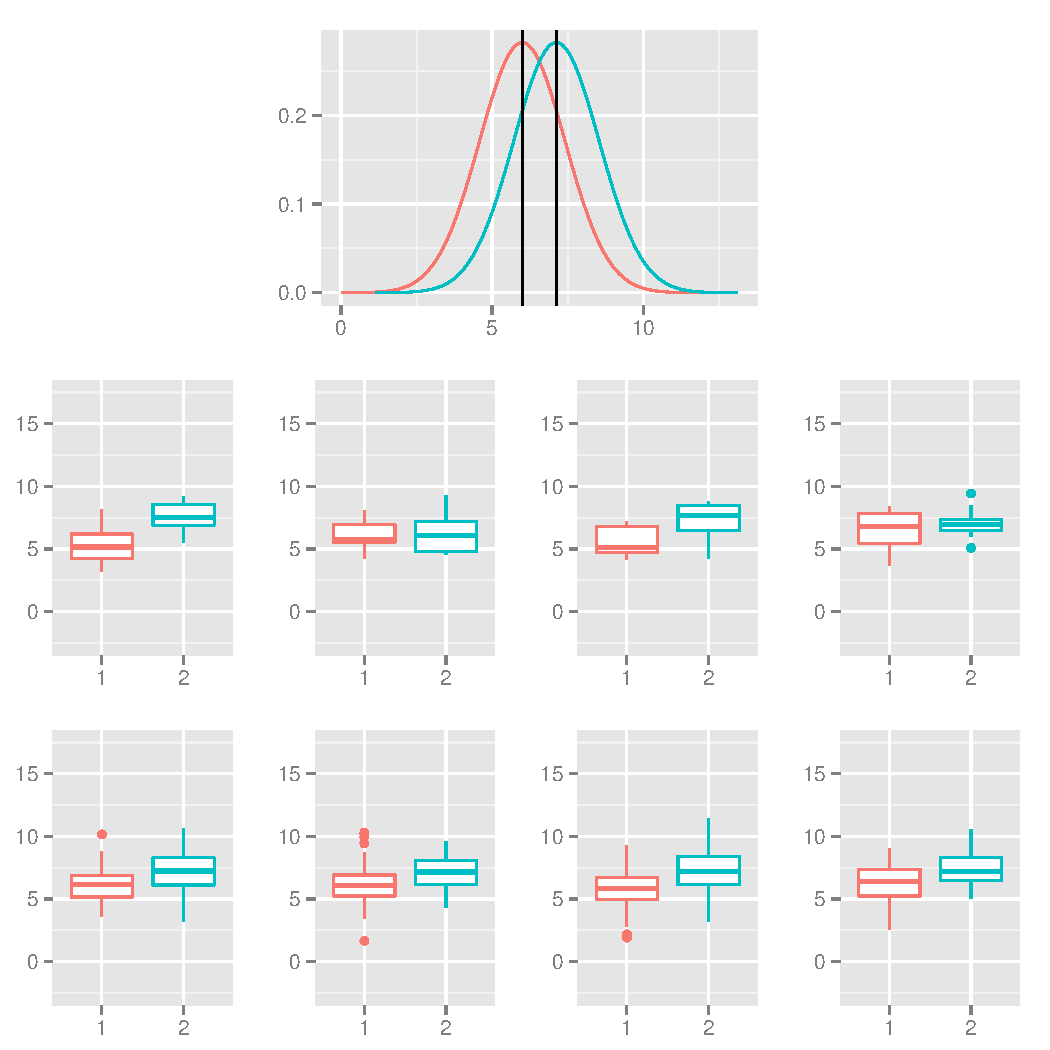
\includegraphics[width=\maxwidth]{figure/varEqualBoxplots} 

\end{knitrout}
\textit{Figure 1.} Boxplots for groups with equal variances. The first row displays groups with $n$=20 and the second row displays groups with $n$=100.
\end{figure}

\begin{figure}
\begin{knitrout}
\definecolor{shadecolor}{rgb}{0.969, 0.969, 0.969}\color{fgcolor}
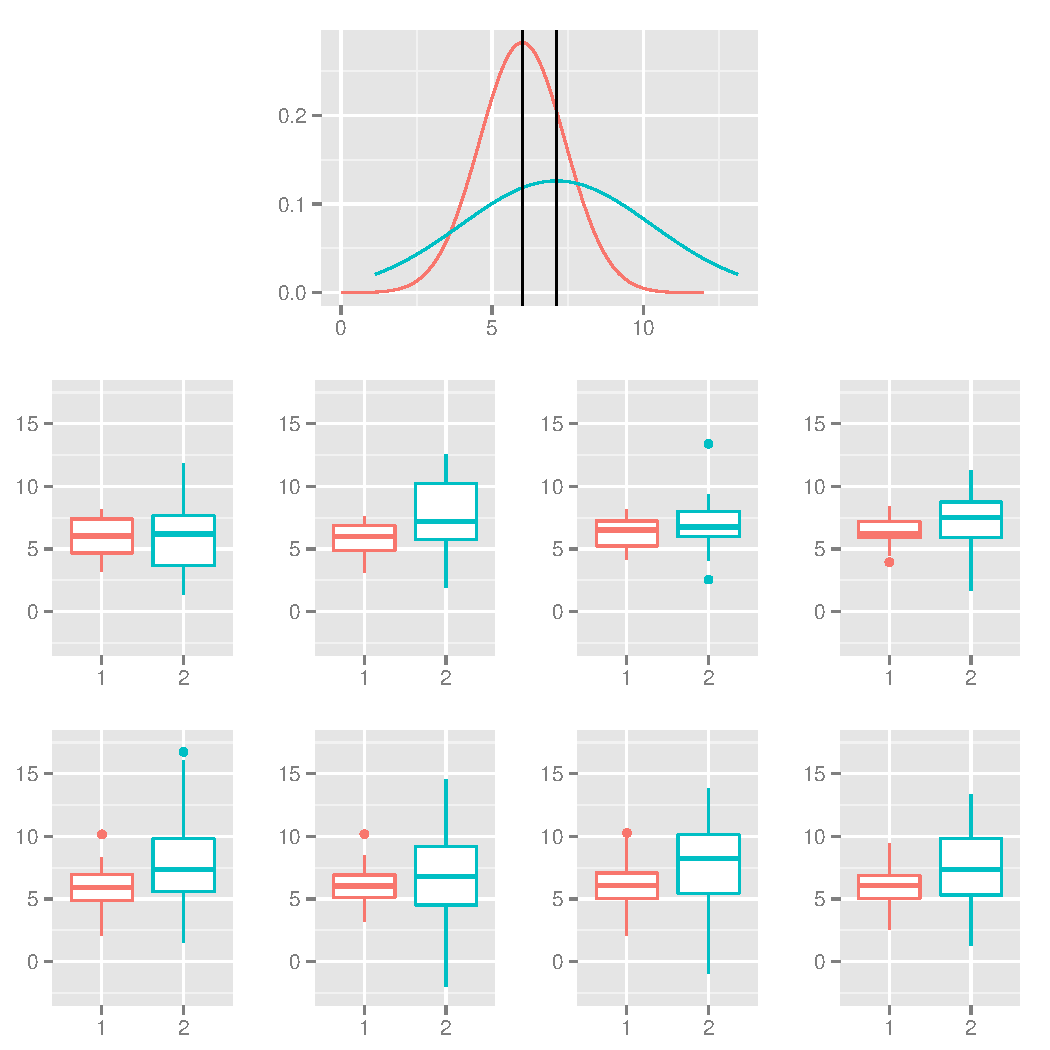
\includegraphics[width=\maxwidth]{figure/varDifferentBoxplots} 

\end{knitrout}
\textit{Figure 2.} Boxplots for groups with unequal variances. The first row displays groups with $n$=20 and the second row displays groups with $n$=100.
\end{figure}


\subsection{Does the df Ratio Help?}
    We examined whether looking at ratio of the Welch t test degrees of freedom to the Student t test degrees of freedom would provide a heuristic for deciding that the equal variances assumption does not hold. Rather than simulate the df ratio, we examined the analytical df ratio as a function of the variance ratio, as a function of the sample size ratio, and as a function of both. 

    Figure 3 displays the change in the df ratio as the variance ratio increases when sample sizes are equal. As expected, the ratio decreases as the difference in variances grows larger. When the variances are equal, the df ratio is equal to 1, though in real data the observed variances will rarely be exactly equal even if the population variances are equal. When once variance is twice the size of the other, the ratio drops to .9. A useful heuristic might to assume that the variances are unequal when the ratio falls below 96\%.
  
\begin{figure}
\begin{knitrout}
\definecolor{shadecolor}{rgb}{0.969, 0.969, 0.969}\color{fgcolor}
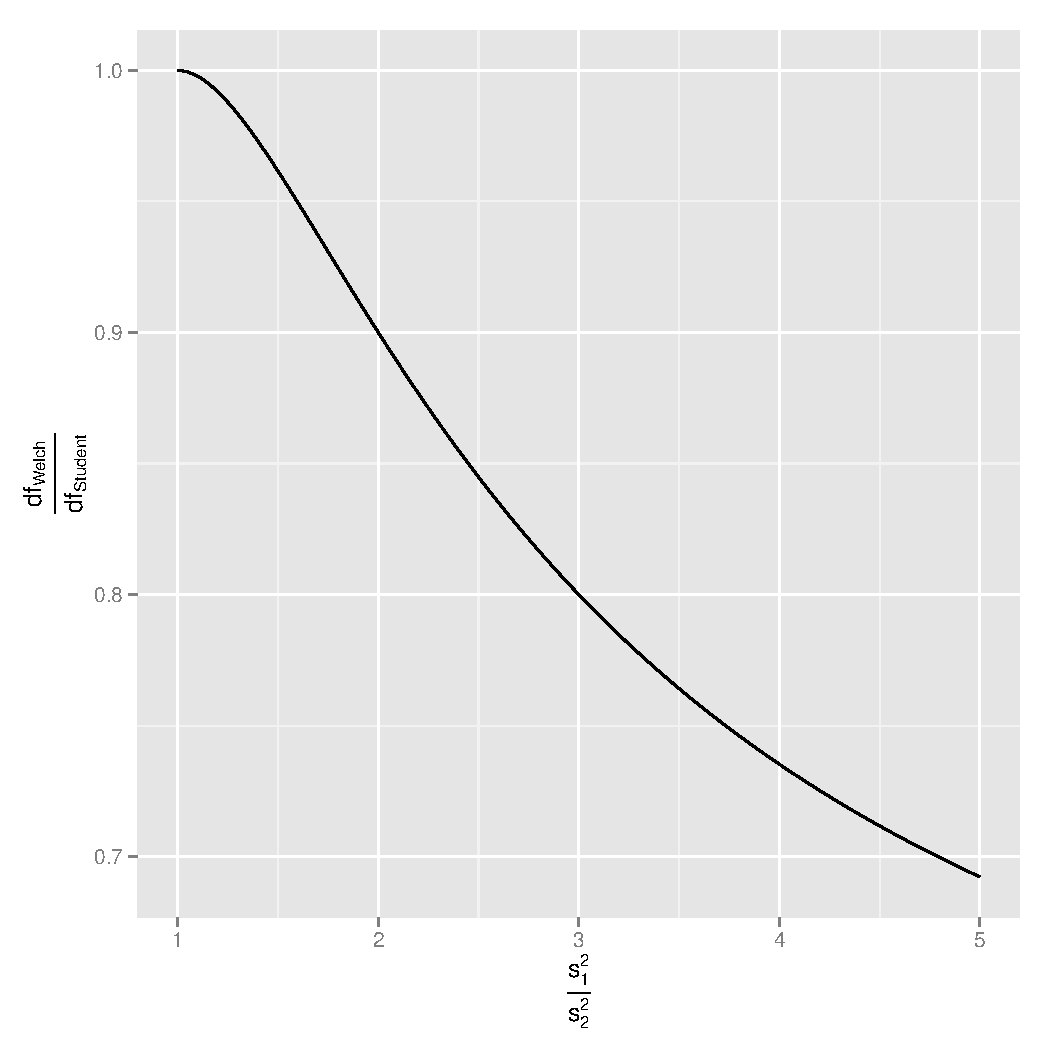
\includegraphics[width=\maxwidth]{figure/dfratiosDiffvars} 

\end{knitrout}
\textit{Figure 3.} Degrees of freedom ratio when sample sizes are equal and variances are unequal.
\end{figure}

    But now look at what happens when the variances are equal and the sample size ratio changes (Figure 4). Here, too, the df ratio decreases as the difference in sample sizes grows larger, even though the variances stay the same. The 96\% heuristic would lead us astray and we would incorrectly conclude that the variances are unequal in many cases when only the sample sizes are unqual.

\begin{figure}
\begin{knitrout}
\definecolor{shadecolor}{rgb}{0.969, 0.969, 0.969}\color{fgcolor}
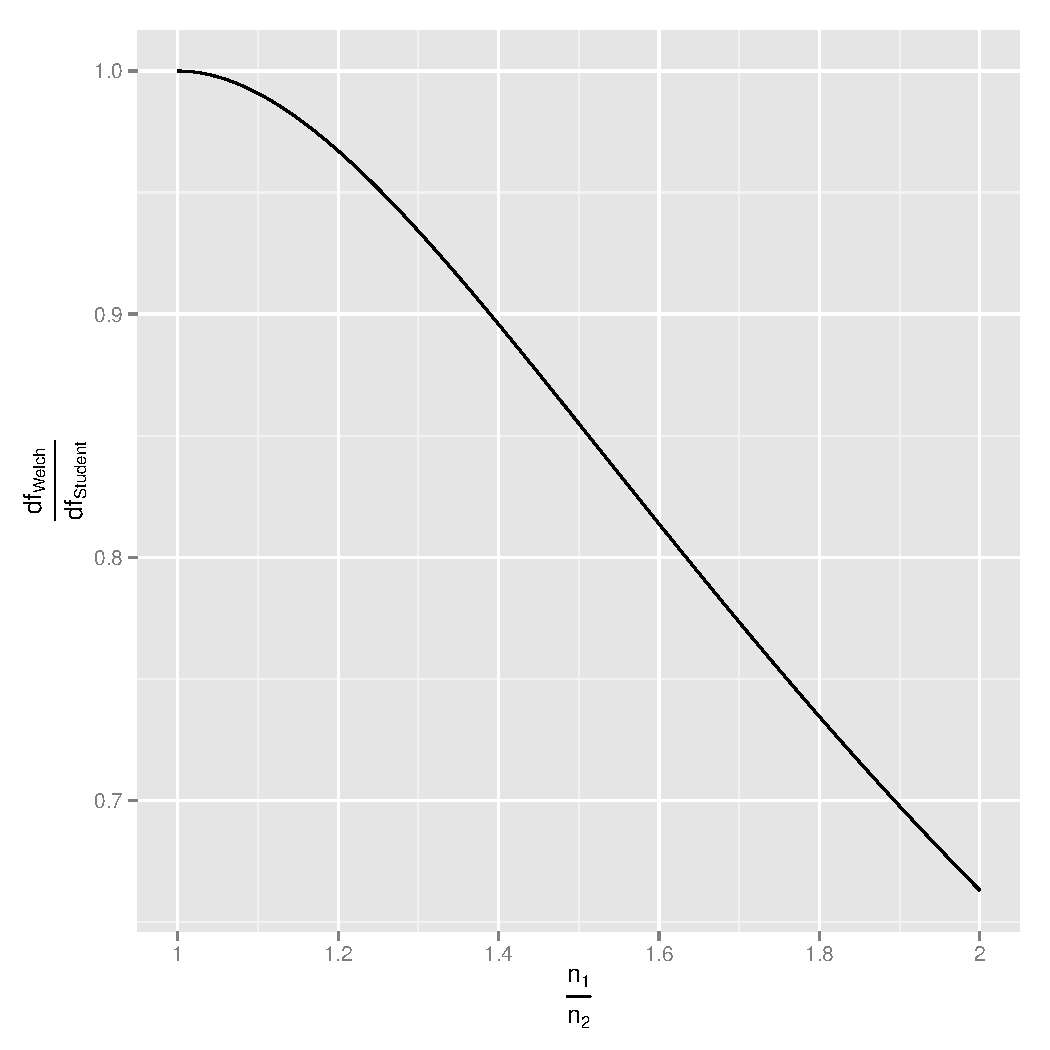
\includegraphics[width=\maxwidth]{figure/dfratiosDiffNratios} 

\end{knitrout}
\textit{Figure 4.} Degrees of freedom ratio when sample sizes are unequal and variances are equal.
\end{figure}

    The picture becomes even more complicated when both the sample sizes and variances are unequal (Figure 5). In this case, the effect of different variances depends on whether the larger group has the larger variance or the smaller variance. When the variance of the larger group is increasing, the move from equal to unequal variances actual counteracts the effect of the unequal sample sizes at first, and the df ratio initially begins to approach 1 before dropping again. Due to the difference in sample sizes, a 96\% heuristic would mislead us into concluding that variances are equal when they are actually three times different from each other. However, when the variance of the smaller group is increasing the immediate drop in the df ratio is quite dramatic before it begins to level off. 

\begin{figure}
\begin{knitrout}
\definecolor{shadecolor}{rgb}{0.969, 0.969, 0.969}\color{fgcolor}
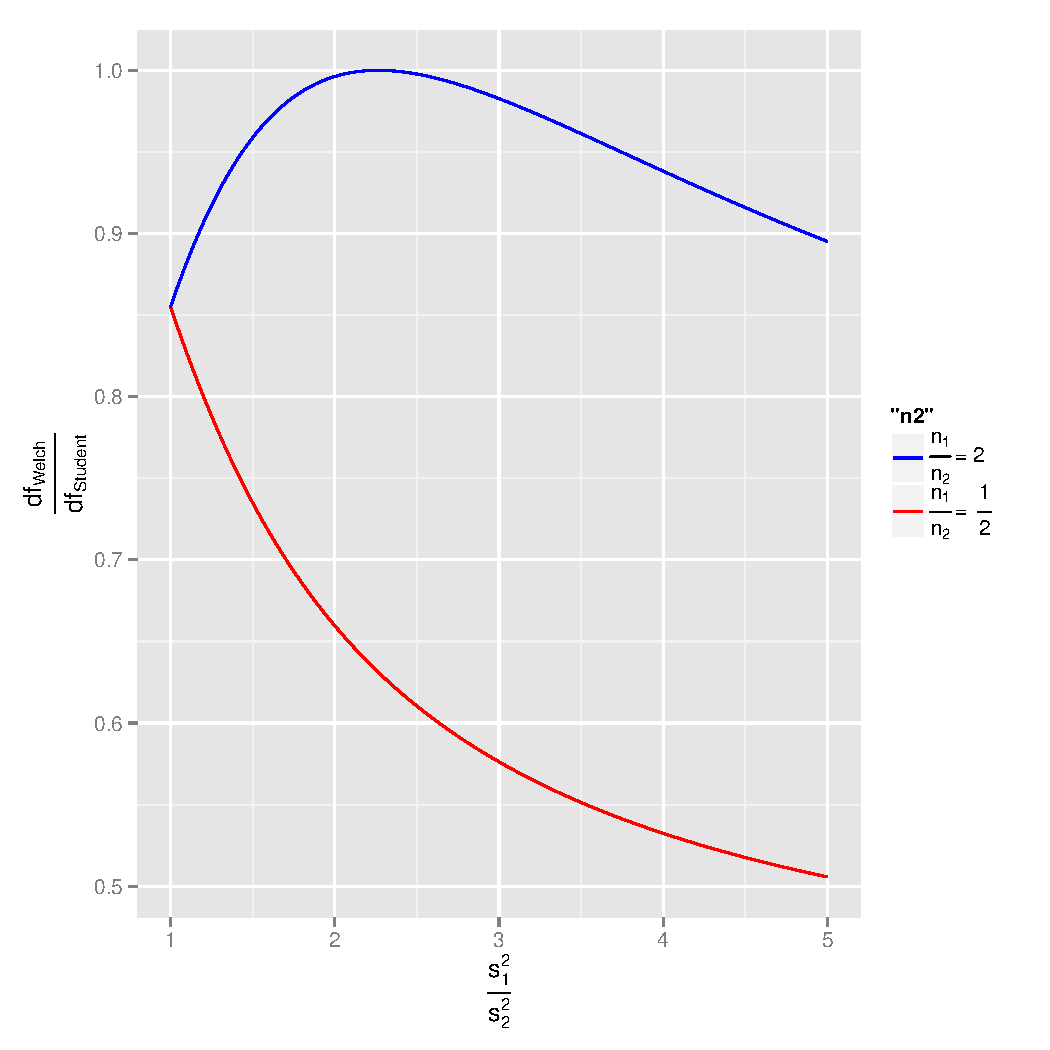
\includegraphics[width=\maxwidth]{figure/dfratiosDiffvarsDiffNratios} 

\end{knitrout}
\textit{Figure 5.} Degrees of freedom ratio when sample sizes are unequal and variances are unequal.
\end{figure}
    In short, the usefulness of a heuristic based on the df ratio is limited to cases when the sample sizes are equal. 

\subsection{When Does Each Test Perform Best?}
    There did not seem to be a simple rule based on the degrees of freedom penalty to detect whether variances are unequal, so we decided to examine when the Welch and Student t tests would perform best based on the sample size, variance ratio, and sample size ratio. We examined how well each test balances the concerns about false positives, power, and estimation. Some prior research has examined the Type I error rate for the two tests \cite{Boneau1960, Zimmerman1993, Zimmerman2004, Zimmerman1996, Zimmerman2009} and some has also examined the power of the two tests, though not always representing the complete configuration of conditions that we examined in our simulations \cite{Neuhauser2002, Zimmerman1993}. Nevertheless, we believe that it will be informative to display the false positives and power of the two tests here. We also discuss implications for effect size estimation, which follows from the false positive results but has not, to our knowledge, been discussed explicitly in past research.

NOTE: Zimmerman1993 only reports power when Student's t test looks bad; Neuhauser only reports power when sample sizes are equal

NOTE: I excluded here citations that looked at ANOVA vs. Welch for now (Overall et al., 1995a, 1995b), but I could add them if we want.
    
\subsubsection{Type I Error Rates}


    The expected type I error rate is $\alpha = .05$. The observed type I error rate for Student's t test remained close to the expected .05 rate when either the sample size or the population variances were equal, but it varied widely when both population variances and sample sizes were unequal (see Figure 7). When the group with the larger sample size had the larger variance (the left side of Figure 7), the type I error rate dropped as low as about .01, but when the group with the larger sample size had the smaller variance (the right side of Figure 7), the type I error rate rose as high as .12, which is more than double the normally accepted false positive rate. In contrast, the observed type I error rate for Welch's t test remained close to the expected .05 rate across all conditions (see Figure 8). Overall, the Welch t test consistently behaved as expected when it comes to false positives. Student's t test did not.

\begin{figure}    
\begin{knitrout}
\definecolor{shadecolor}{rgb}{0.969, 0.969, 0.969}\color{fgcolor}
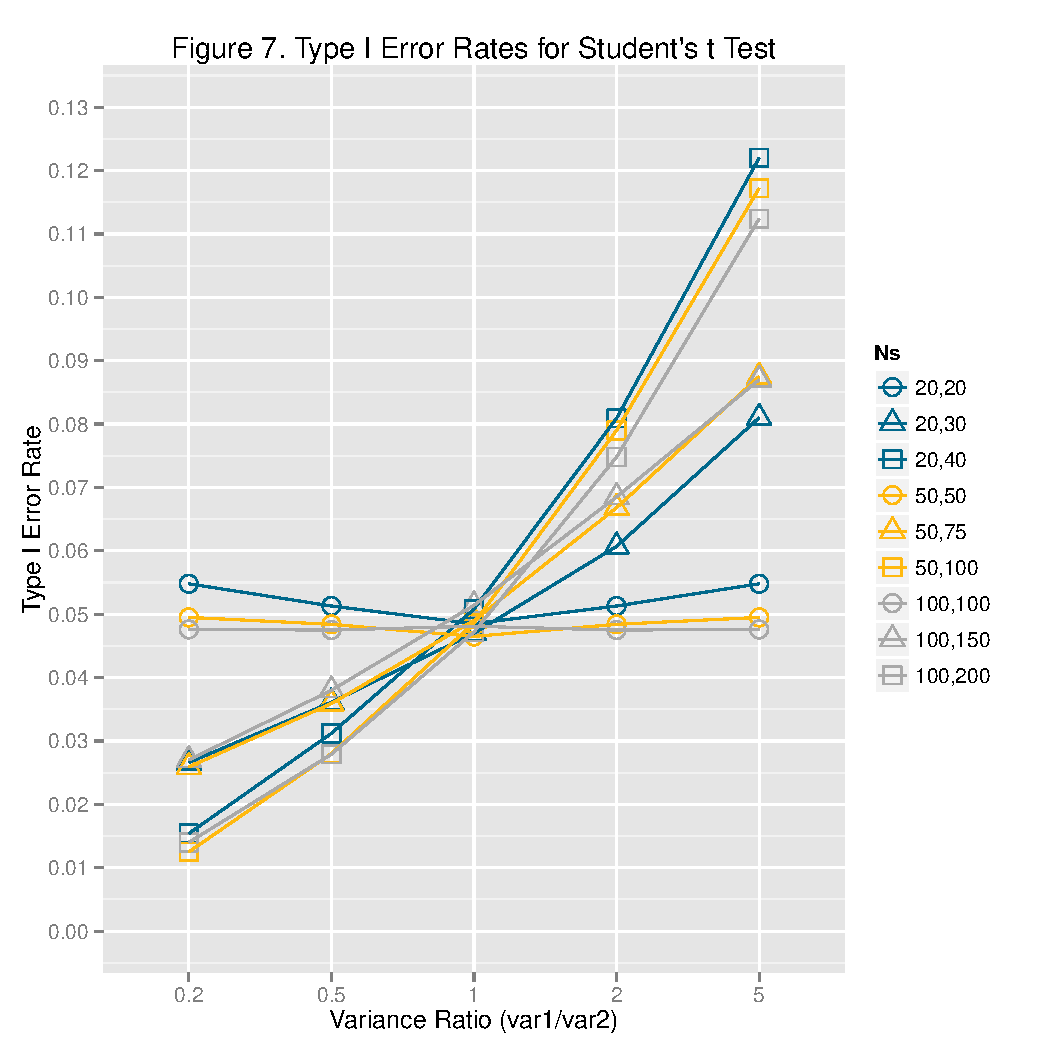
\includegraphics[width=\maxwidth]{figure/type1_classic_plot} 

\end{knitrout}
\textit{Figure 7.} Type I error rates for Student's t test.
\end{figure}


\begin{figure}
\begin{knitrout}
\definecolor{shadecolor}{rgb}{0.969, 0.969, 0.969}\color{fgcolor}
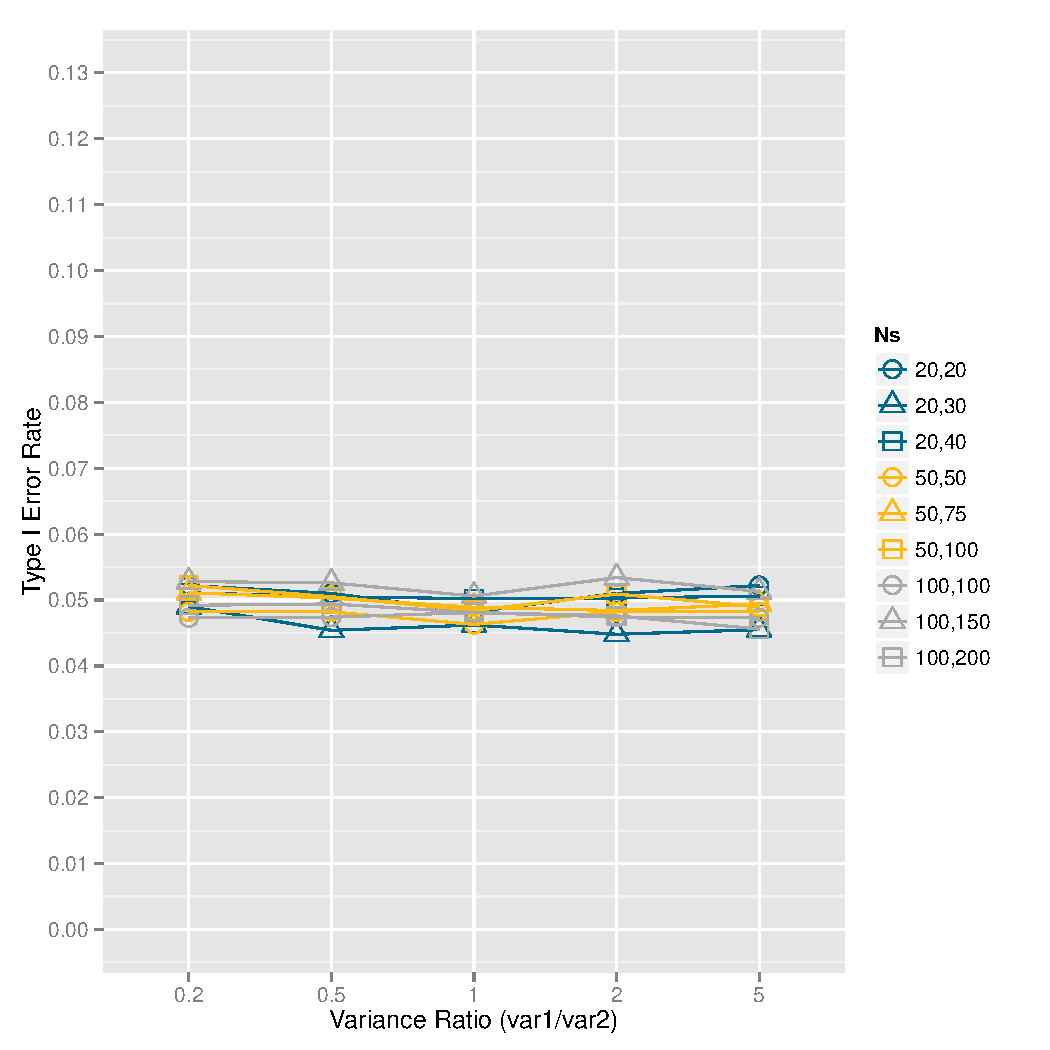
\includegraphics[width=\maxwidth]{figure/type1_Welch_plot} 

\end{knitrout}
\textit{Figure 8.} Type I error rates for Welch's t test.
\end{figure}

\subsubsection{Power}






    Is Welch's t test underpowered compared to Student's t test? Figure 9 displays the power of Student's t test and of Welch t tests to detect small, medium, and large effects under the different conditions. For both tests, power decreases as variances become unequal because we increased one group's variance; however, the power of each test decreases at a different rate depending on the sample size ratio. Figure 10 displays the difference in power between Student's t test and Welch's t test, with higher numbers indicating that Student's t test is more powerful. When the sample sizes or variances are equal, the power of the two tests is approximately equal. However, when both the sample sizes and variances are unequal, there are differences in power. Overall, Student's t test is more powerful when the large sample has the smaller variance, whereas the Welch t test is more powerful when the small sample has the smaller variance. These differences are the most dramatic when one sample is twice the size of the other. 
    
    The conditions in which Student's t test has the greatest power over Welch's t test, when one sample is twice the size of the other and the large sample has the small variance, are the same conditions in which Student's t test has a risk of doubling the false positive rate. In contrast, Welch's t test was more powerful than Student's t test under other conditions and never inflated the type I error rate beyond the expected rate.

    Taken together, the type I error rates and power favor the Welch t test over Student's t test as better balancing researchers' concerns.
\begin{figure}
\begin{knitrout}
\definecolor{shadecolor}{rgb}{0.969, 0.969, 0.969}\color{fgcolor}
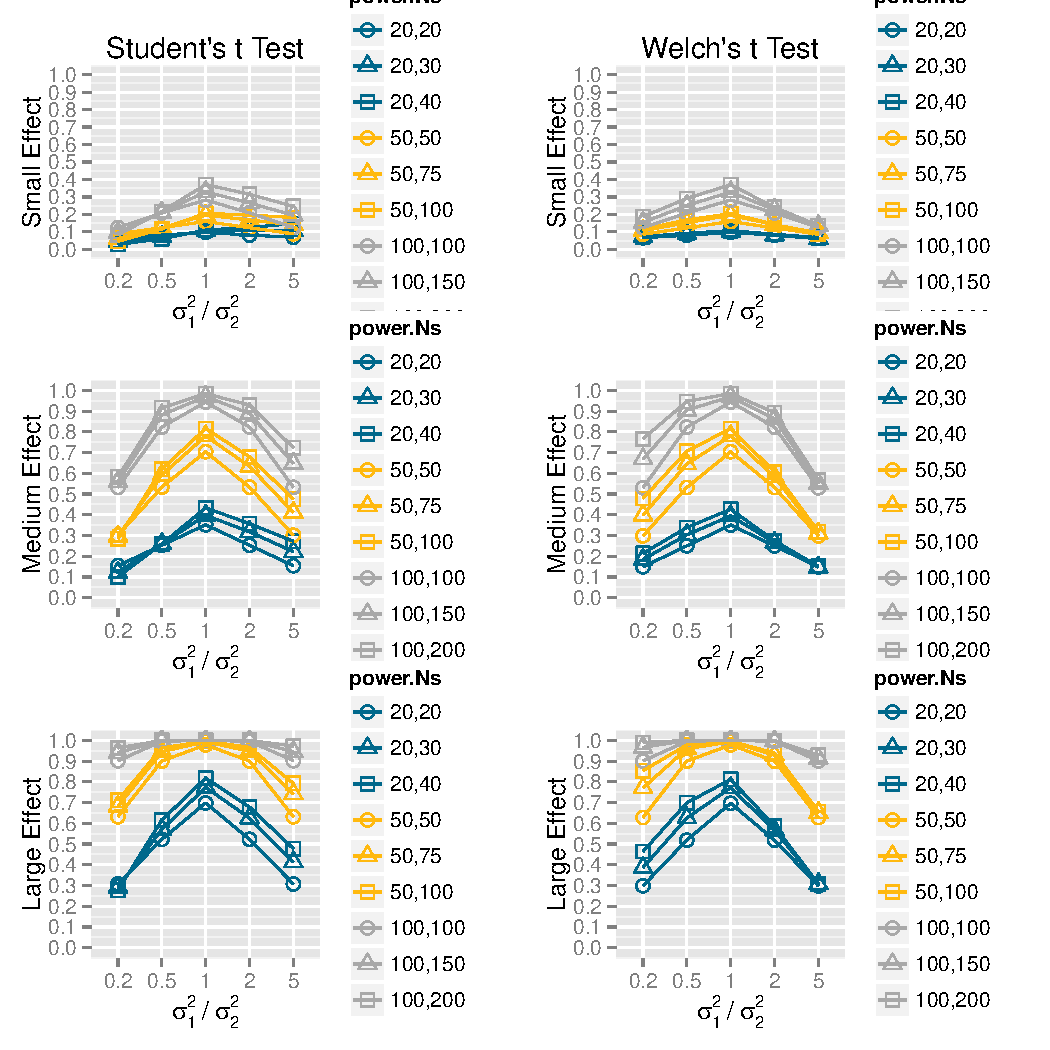
\includegraphics[width=\maxwidth]{figure/plotPower} 

\end{knitrout}
\textit{Figure 9.} Power of Student's and Welch's t tests.
\end{figure}

\begin{figure}
\begin{knitrout}
\definecolor{shadecolor}{rgb}{0.969, 0.969, 0.969}\color{fgcolor}
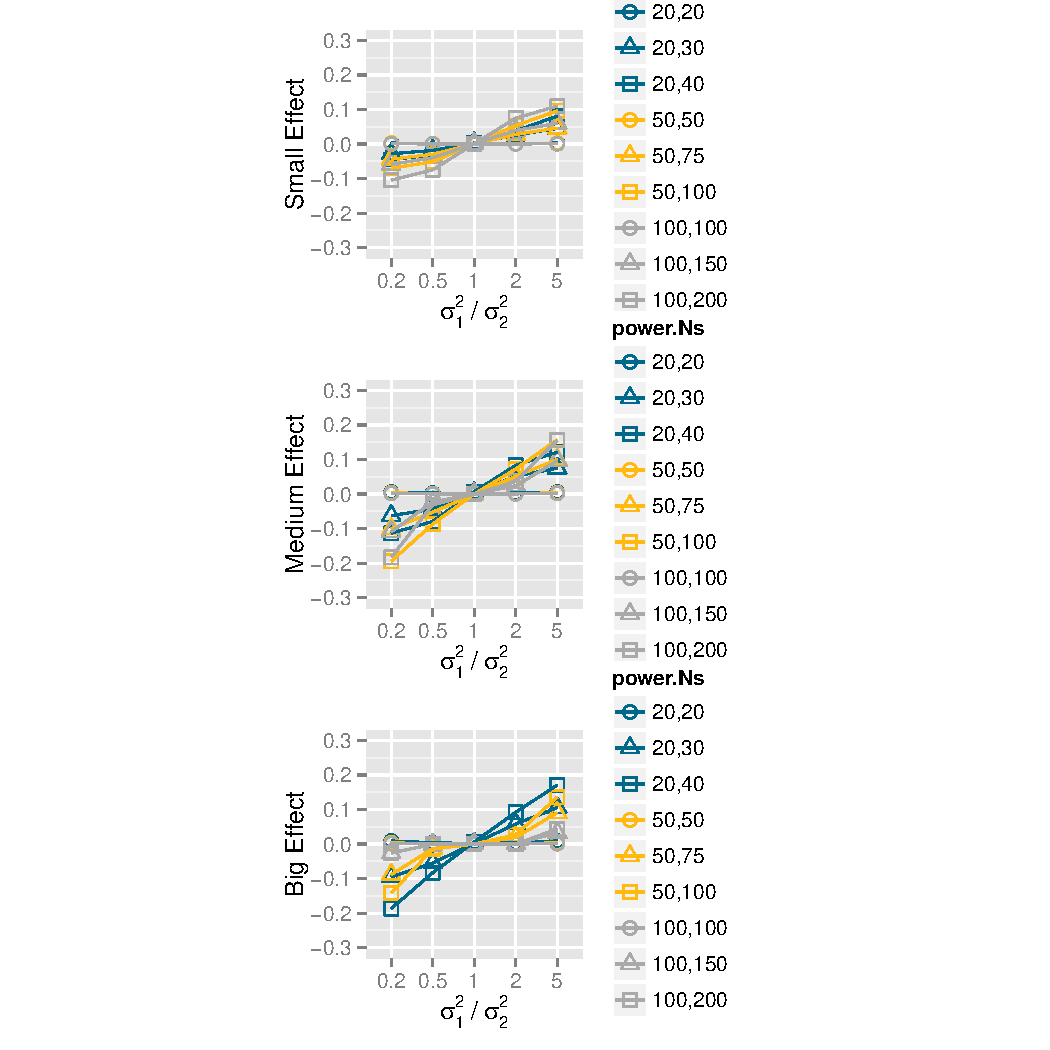
\includegraphics[width=\maxwidth]{figure/plotPowerDiff} 

\end{knitrout}
\textit{Figure 10.} Difference in the Power of Student's and Welch's t tests (Student-Welch).
\end{figure}

\subsubsection{Coverage Probability}
Because the accuracy of a confidence interval is influenced by the variance and sample size, but not by the true effect size, we only show the coverage probability when the null hypothesis is true (the coverage probabilities are identical across all effect sizes). Table 10 displays the coverage probability, which is how often the 95\% confidence interval contains the true mean difference in groups, for the two tests under the different conditions. The coverage probability for the classic t test varies dramatically. When it is the least powerful, it is the most accurate. When it is the most powerful, the effect size estimation is the least accurate, and what seems to be a 95\% confidence interval drops as low as an 88\% confidence interval. Once again, the Welch t test retains the expected 95\% rate and turns out to best meet a researcher's concerns. 






\begin{figure}
\begin{knitrout}
\definecolor{shadecolor}{rgb}{0.969, 0.969, 0.969}\color{fgcolor}
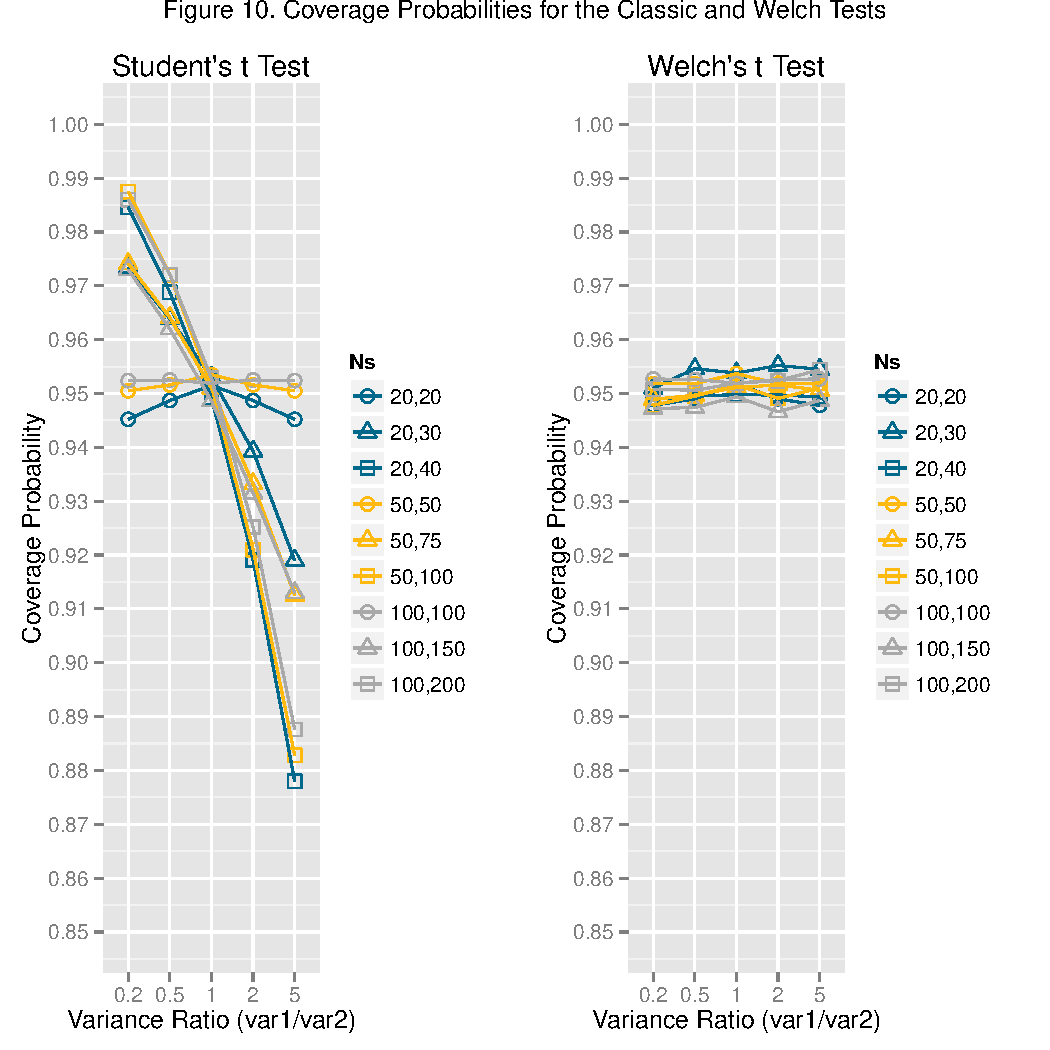
\includegraphics[width=\maxwidth]{figure/coverage_plots} 

\end{knitrout}
\textit{Figure 10.} Coverage probabilities for Student's and Welch's t tests.
\end{figure}

\section{Discussion}
    Make a note that our df ratio rule works best when it doesn't matter - when sample sizes are equal.
    
    In much experimental work, the choice between the tests is probably fine if the experimenter ensures that sample sizes are equal. This is generally not an option with pre-existing groups. 
    
    Notably, the two standard errors are equal when either the sample sizes or the variances of the two groups are identical, so the Welch t test could only be more powerful when both the sample sizes and variances are unequal. 
    
    Benefits of just using welch rule: simplifies the decision which makes it easier, puts researcher motivation in line with false positive preservation

    One of the concerns about using the Welch t test as an alternative to Student's t test is that the penalty on the degrees of freedom makes it difficult to find effects. Figures 3 and 4 show that the penalty is small when the variances and sample sizes are approximately equal, which is within the range that one might expect from normal sampling error when the true population variances are equal. However, the penalty to the degrees of freedom might not be very important in general. Figure 6 displays two t-distributions where one has half the degrees of freeom of the other. Despite the drastic difference in the degrees of freedom, the two distributions largely overlap and so the differences in standard errors of the two tests, which will affect the value of the t-test, might be more important.
    
    Cite Zimmerman 1996 when talking about how the pooled variance is the major cause of problems with Student's t test
    
    Cohen's d is a population standardized mean difference based on the standard deviation of the population - but what if there is no standard deviation of the population? This is exactly the situation we're faced with when lifting the equal variances assumption.
  
\begin{figure}  
\begin{knitrout}
\definecolor{shadecolor}{rgb}{0.969, 0.969, 0.969}\color{fgcolor}
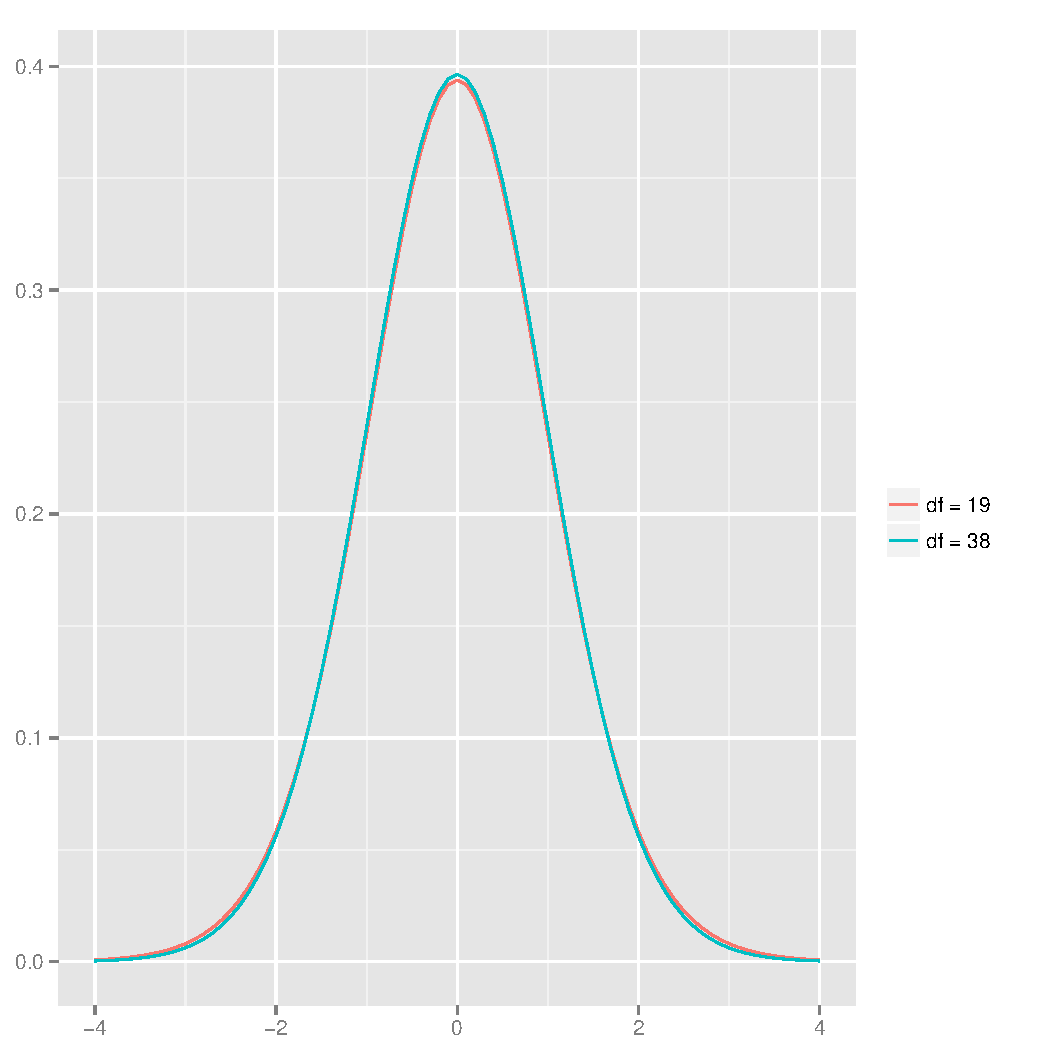
\includegraphics[width=\maxwidth]{figure/tdist} 

\end{knitrout}
\textit{Figure 6. Two t distributions with different degrees of freedom.}
\end{figure}




\bibliography{bibliography}
\bibliographystyle{apacite}

\end{document}
